\documentclass[tikz,border=2pt]{standalone}
\begin{document}
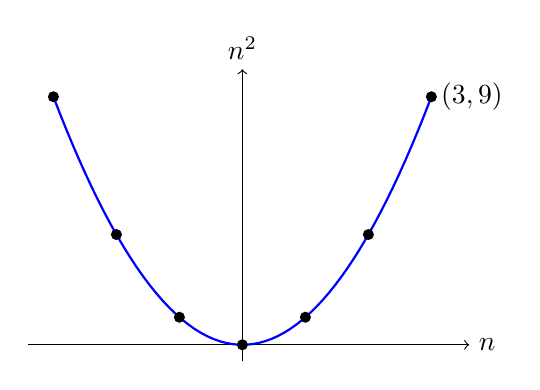
\begin{tikzpicture}[x=0.8cm,y=0.35cm]
  \draw[->] (-3.4,0) -- (3.6,0) node[right] {$n$};
  \draw[->] (0,-0.6) -- (0,10) node[above] {$n^2$};
  \draw[blue, thick, domain=-3:3, samples=60] plot (\x,{\x*\x});
  \foreach \n in {-3,...,3} \fill (\n,{\n*\n}) circle (2pt);
  \node[right] at (3,9) {$(3,9)$};
\end{tikzpicture}
\end{document}
